\documentclass[11pt,a4paper]{article}
\usepackage[margin=2.5cm]{geometry}
\usepackage{times}
\usepackage{hyperref}
\usepackage{natbib}
\renewcommand{\bibsection}{\section*{References}}
\usepackage{latexsym}
\usepackage{amsmath}
\usepackage{amssymb}
\usepackage{graphicx}
\usepackage{booktabs}
\usepackage{multirow}
\usepackage{xcolor}
\usepackage{pgfplots}
\pgfplotsset{compat=1.17}
\usepackage{tikz}
\usepackage{subcaption}

\title{Structural Consistency for Confidence Estimation in\\LLM-Based Information Extraction:\\A Systematic Comparison and the Correlation-Selection Gap}

\author{Anonymous}

\begin{document}
\maketitle

\begin{abstract}
Multi-sample generation with large language models (LLMs) is increasingly used for structured prediction tasks such as named entity recognition (NER) and relation extraction (RE), yet practitioners lack principled guidance on which confidence signals to trust---and for what purpose.
We present the first systematic comparison of five unsupervised confidence signals across four families for LLM-based information extraction: model log-probability, surface-level agreement (Fleiss' Kappa, exact match), and two structural consistency measures (soft Jaccard similarity, entity-level majority voting).
On two NER datasets (SciERC, CoNLL-2003) with two models (Qwen3-8B, LLaMA-3.1-8B), structural consistency signals provide the strongest instance-level quality estimation, with entity voting achieving AUROC 0.73 and $\rho{=}0.50$ on SciERC NER---far above log-probability (AUROC 0.56, $\rho{=}0.14$).
However, we identify a \emph{correlation-selection gap}: despite strong instance-level correlation, \textbf{no} unsupervised signal beats greedy decoding for NER best-of-$N$ selection, while large oracle headroom (+16pp F1) exists.
On RE, only log-probability enables marginal selection improvement (+0.7pp), while all signals degrade due to compound error propagation.
We provide a practical decision framework: use structural consistency for selective prediction and abstention; use log-probability for best-of-$N$ selection on tasks where greedy is suboptimal; and for closed-source APIs where log-probabilities are unavailable, structural consistency offers the only viable confidence signal.
\end{abstract}

%=============================================================
\section{Introduction}
\label{sec:intro}
%=============================================================

Test-time scaling (TTS)---generating multiple candidate outputs and selecting the best---has emerged as a powerful strategy for improving LLM reasoning~\cite{wang2023selfconsistency,snell2024scaling,brown2024large}.
For reasoning tasks with discrete answers, self-consistency via majority voting reliably improves accuracy.
But for \emph{structured prediction} tasks---named entity recognition (NER) and relation extraction (RE)---the outputs are \emph{sets} of typed spans and relations, not single tokens.
How should practitioners assess the quality of such structured outputs, and can multi-sample generation improve them?

Prior work on LLM confidence estimation has largely focused on free-form generation~\cite{kuhn2023semantic,manakul2023selfcheckgpt,kadavath2022language} or classification~\cite{guo2017calibration,desai2020calibration}.
For structured IE, \citet{nédellec2026consistency} recently studied consistency--accuracy correlations for entity and relation extraction, but used surface-level string matching and acknowledged this ``overlooks semantically consistent outputs.''
Test-time scaling methods such as CISC~\cite{huang2025cisc}, Self-Certainty Best-of-$N$~\cite{zhang2026selfcertainty}, and ReASC~\cite{li2026reasc} target reasoning tasks with discrete answers, leaving structured prediction unexplored.

We address this gap with a systematic empirical comparison of five unsupervised confidence signals across four families for LLM-based IE (Figure~\ref{fig:overview}).
Our taxonomy spans: (1)~\emph{model confidence} (sequence log-probability), (2)~\emph{surface agreement} (Fleiss' Kappa, exact match), (3)~\emph{set-aware structural similarity} (soft Jaccard over entity sets), and (4)~\emph{entity-level majority voting confidence}.
We evaluate each signal for two distinct purposes that prior work has conflated: \emph{instance-level quality estimation} (predicting which inputs yield reliable outputs) and \emph{per-sample selection} (choosing the best output among $N$ candidates).

Our contributions are:
\begin{enumerate}
\item A systematic empirical comparison showing structural consistency signals (voting, soft Jaccard) are the strongest quality estimators for IE, significantly outperforming log-probability ($\Delta$AUROC up to +0.17).
    The contribution lies in the taxonomy and comparative methodology, not in any individual signal.
\item The identification of a \textbf{correlation-selection gap}: strong instance-level quality estimation ($\rho{\approx}0.50$) does not translate to effective best-of-$N$ selection.
    We provide concrete practical guidance via a decision flowchart (Section~\ref{sec:practical}).
\item An empirical analysis of task-complexity boundaries, showing compound error propagation in relational tasks degrades all confidence signals, with per-relation-type heterogeneity ranging from $\rho{=}0.55$ (HYPONYM-OF) to $\rho{=}0.00$ (FEATURE-OF).
\end{enumerate}

\begin{figure}[t]
\centering
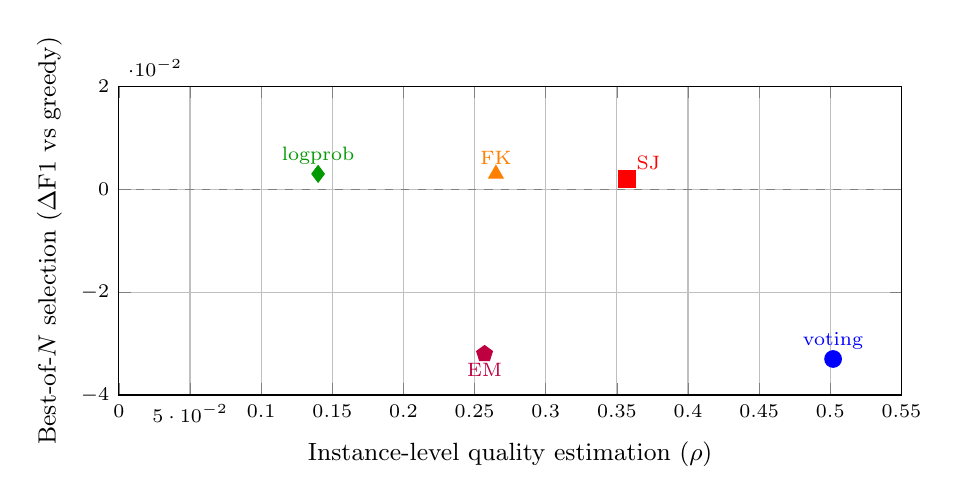
\begin{tikzpicture}
\begin{axis}[
  width=0.95\columnwidth, height=5.5cm,
  xlabel={Instance-level quality estimation ($\rho$)},
  ylabel={Best-of-$N$ selection ($\Delta$F1 vs greedy)},
  xmin=0, xmax=0.55, ymin=-0.04, ymax=0.02,
  grid=major,
  legend style={at={(0.02,0.02)},anchor=south west,font=\scriptsize},
  every axis label/.style={font=\small},
  tick label style={font=\scriptsize},
]
\addplot[only marks, mark=*, mark size=3pt, blue] coordinates {(0.502,-0.033)};
\addplot[only marks, mark=square*, mark size=3pt, red] coordinates {(0.357,0.002)};
\addplot[only marks, mark=triangle*, mark size=3pt, orange] coordinates {(0.265,0.003)};
\addplot[only marks, mark=diamond*, mark size=3pt, green!60!black] coordinates {(0.140,0.003)};
\addplot[only marks, mark=pentagon*, mark size=3pt, purple] coordinates {(0.257,-0.032)};
\draw[dashed, gray] (axis cs:0,0) -- (axis cs:0.55,0);
\node[font=\scriptsize, blue, anchor=south] at (axis cs:0.502,-0.033) {voting};
\node[font=\scriptsize, red, anchor=south west] at (axis cs:0.357,0.002) {SJ};
\node[font=\scriptsize, orange, anchor=south] at (axis cs:0.265,0.003) {FK};
\node[font=\scriptsize, green!60!black, anchor=south] at (axis cs:0.140,0.003) {logprob};
\node[font=\scriptsize, purple, anchor=north] at (axis cs:0.257,-0.032) {EM};
\end{axis}
\end{tikzpicture}
\caption{The correlation-selection gap on SciERC NER ($N{=}16$). $x$-axis: instance-level quality estimation (Spearman $\rho$ with F1). $y$-axis: best-of-$N$ selection gain over greedy. Signals with strong quality estimation (voting, SJ) fail at selection; the dashed line marks greedy performance. Oracle headroom is +16.9pp.}
\label{fig:overview}
\end{figure}

%=============================================================
\section{Related Work}
\label{sec:related}
%=============================================================

\paragraph{Uncertainty Quantification for LLMs.}
Uncertainty estimation in LLMs has been extensively surveyed~\cite{geng2025uqsurvey,hou2025uqcalibsurvey,xiong2024confestimation,yoshikawa2025abstention}.
Approaches include token-level log-probabilities~\cite{kadavath2022language}, semantic entropy over meaning clusters~\cite{kuhn2023semantic}, semantic entropy probes for efficient estimation~\cite{kossen2024semanticprobes}, and sampling-based methods such as SelfCheckGPT~\cite{manakul2023selfcheckgpt}.
For calibration, \citet{guo2017calibration} established that modern neural networks are poorly calibrated; \citet{desai2020calibration} and \citet{kuleshov2015calibration} extended this to NLP.
Our work differs by focusing on \emph{structured set-valued} outputs where token-level confidence is insufficient.

\paragraph{Self-Consistency and Test-Time Scaling.}
\citet{wang2023selfconsistency} showed majority voting over chain-of-thought samples improves reasoning accuracy.
Recent extensions include CISC~\cite{huang2025cisc} (confidence-weighted voting), Self-Certainty Best-of-$N$~\cite{zhang2026selfcertainty} (KL-divergence reward-free selection), ReASC~\cite{li2026reasc} (reliability-aware adaptive consistency), Atomic Self-Consistency~\cite{chen2024atomic} (sub-claim decomposition), Ranked Voting~\cite{liu2025rankedvoting}, and Latent Self-Consistency~\cite{wu2025latentsc} (embedding-space agreement).
\citet{snell2024scaling} and \citet{brown2024large} analyze TTS scaling laws.
Verifier-based approaches~\cite{cobbe2021verifier,lightman2023stepwise} train reward models for selection.
All of these target reasoning/QA with discrete answers; we are the first to systematically compare confidence signals for \emph{structured IE} and to identify the correlation-selection gap.

\paragraph{Confidence and Consistency for Structured IE.}
\citet{nédellec2026consistency} study consistency--accuracy correlations for entity and relation extraction using surface-level string matching across four LLMs, acknowledging this approach ``overlooks semantically consistent outputs.''
Our soft Jaccard metric addresses exactly this limitation.
\citet{culotta2004confidence} estimated confidence for traditional CRF-based IE.
\citet{xiao2019uncertainty} and \citet{shelmanov2021uncertainty} study uncertainty in sequence labeling.
\citet{jagannatha2022calibration} address structured calibration.
For ensemble/MC-dropout uncertainty, see \citet{lakshminarayanan2017simple} and \citet{gal2016dropout}.
CoCoA~\cite{vashurin2025cocoa} integrates confidence and consistency within an MBR framework for QA/summarization but does not address structured IE.
\citet{geifman2017selective} formalize selective prediction, directly relevant to our quality estimation application.

%=============================================================
\section{Method}
\label{sec:method}
%=============================================================

\subsection{Problem Setup}

Given an input $x$ and a generative LLM, we sample $N$ structured outputs $\{y_1, \ldots, y_N\}$ at temperature $T{>}0$.
Each output $y_i$ is a set of entities (for NER) or a set of (head, relation, tail) triples (for RE).
We also obtain a greedy output $y^*$ at $T{=}0$.
The goal is twofold: (1)~\emph{quality estimation}: predict the quality (F1 score) of the greedy output $y^*$ using information from the $N$ stochastic samples; (2)~\emph{sample selection}: select the highest-quality sample from $\{y_1, \ldots, y_N\}$.

\subsection{Confidence Signals}

We evaluate five signals across four families:

\paragraph{(1) Log-probability (logprob).}
The normalized sequence log-probability of each sample: $s_{\text{lp}}(y_i) = \frac{1}{|y_i|}\sum_{t} \log p(y_{i,t} \mid y_{i,<t}, x)$.
This is the only \emph{per-sample} signal---it assigns different scores to different samples $y_i$, enabling direct best-of-$N$ selection.

\paragraph{(2) Exact Match rate (EM).}
The fraction of sample pairs with identical string outputs: $s_{\text{EM}} = \binom{N}{2}^{-1} \sum_{i<j} \mathbb{1}[y_i = y_j]$.
This is the direct analog of self-consistency voting~\cite{wang2023selfconsistency} applied to structured outputs.

\paragraph{(3) Fleiss' Kappa (FK).}
Inter-annotator agreement across $N$ samples, treating each sample as an annotator. Computed at the entity level for NER and the triple level for RE.

\paragraph{(4) Soft Jaccard Similarity (SJ).}
A set-aware structural similarity that accounts for partial matches between entity sets.
For two entity sets $A$ and $B$, we compute an optimal matching via type-grouped Hungarian assignment, then:
\begin{equation}
\text{SJ}(A, B) = \frac{\sum_{(a,b) \in M} \text{overlap}(a,b)}{\max(|A|, |B|)}
\end{equation}
where $M$ is the matching and $\text{overlap}$ measures span overlap within each entity type.
The instance-level SJ score averages over all $\binom{N}{2}$ sample pairs.
To avoid evaluation circularity, we use leave-one-out SJ: each sample's score is the mean SJ with the remaining $N{-}1$ samples (max $\Delta\rho = 0.0003$ vs full SJ).

\paragraph{(5) Entity Voting Confidence (voting\_conf).}
For each entity mention extracted in any sample, we compute the fraction of $N$ samples containing that entity (with fuzzy span matching).
The instance-level score averages entity-level voting fractions weighted by entity frequency.
Like SJ, this is an \emph{instance-level aggregate}---it produces one score per input instance, not per sample.

\paragraph{Instance-level vs.\ Per-sample Signals.}
A critical distinction: signals (2)--(5) are \emph{instance-level aggregates} that produce a single confidence score per input instance $x$.
They predict \emph{which inputs are easy/hard} but cannot rank individual samples $y_i$ against each other.
Only log-probability (1) is a \emph{per-sample signal} that can rank candidates for selection.
This distinction explains the correlation-selection gap we identify.

\subsection{Evaluation Protocol}

\paragraph{Quality Estimation.}
We measure rank correlation (Spearman $\rho$, Kendall $\tau$) and discriminative ability (AUROC, with median F1 as threshold) between each signal and the greedy output's entity-level F1 score.

\paragraph{Sample Selection.}
We evaluate best-of-$N$ selection: for each instance, select the sample with the highest signal score and report its F1.
For instance-level signals, all samples from the same instance share the same score, so selection is equivalent to random choice---these signals \emph{cannot} perform sample selection by design.
We compare against greedy decoding ($T{=}0$), random selection, and oracle (best possible sample).

\paragraph{Conditional Evaluation.}
To separate model capability gaps from genuine uncertainty, we report results on the \emph{conditional set}: instances where at least one sample achieves $\text{F1} > 0$, excluding cases where the model systematically fails.

%=============================================================
\section{Experimental Setup}
\label{sec:setup}
%=============================================================

\paragraph{Datasets.}
We use SciERC~\cite{luan2018scierc} (scientific text, 6 entity types, 7 relation types; $n_{\text{NER}}{=}529$, $n_{\text{RE}}{=}397$) and CoNLL-2003~\cite{tjong2003conll} (news text, 4 entity types; $n{=}2{,}756$).
We also attempted WNUT-17~\cite{derczynski2017wnut} (social media NER) but abandoned it: 54\% of samples had F1=0, indicating model capability failure rather than uncertainty.

\paragraph{Models.}
Qwen3-8B and LLaMA-3.1-8B, both instruction-tuned, used in a zero-shot structured extraction prompt.
Sampling at $T{=}1.0$ with $N{=}8$ (primary) and $N{=}16$ (scaling analysis), three random seeds for robustness.

\paragraph{Evaluation.}
Entity-level micro-F1 as the ground-truth quality metric.
We report Spearman $\rho$, Kendall $\tau$, and AUROC for quality estimation; F1 for best-of-$N$ selection.

%=============================================================
\section{Results}
\label{sec:results}
%=============================================================

\subsection{Quality Estimation: Structural Signals Dominate}
\label{sec:qe}

Table~\ref{tab:unified} presents unified quality estimation results on SciERC.
On NER, entity voting confidence achieves the highest correlation ($\rho{=}0.502$, AUROC${=}0.728$), followed by soft Jaccard ($\rho{=}0.357$, AUROC${=}0.666$).
Both substantially outperform log-probability ($\rho{=}0.140$, AUROC${=}0.559$), with the structural-vs-surface AUROC gap reaching 0.17 (voting vs logprob).

On RE, the pattern partially holds: voting confidence leads ($\rho{=}0.422$, AUROC${=}0.716$), but log-probability ($\rho{=}0.247$, AUROC${=}0.635$) outperforms SJ ($\rho{=}0.211$, AUROC${=}0.582$) on the full set.
This reversal on RE is explained by compound error propagation (Section~\ref{sec:diagnostic}).
On the conditional set (instances where at least one sample has F1$>$0), SJ recovers to $\rho{=}0.368$, substantially above logprob ($\rho{=}0.146$).

\begin{table}[t]
\centering
\small
\caption{Unified quality estimation on SciERC ($N{=}8$, $T{=}1.0$). Spearman $\rho$, Kendall $\tau$, and AUROC. Best in \textbf{bold}, second \underline{underlined}.}
\label{tab:unified}
\begin{tabular}{l ccc ccc}
\toprule
& \multicolumn{3}{c}{\textbf{NER} ($n{=}529$)} & \multicolumn{3}{c}{\textbf{RE} ($n{=}397$)} \\
\cmidrule(lr){2-4}\cmidrule(lr){5-7}
Signal & $\rho$ & $\tau$ & AUROC & $\rho$ & $\tau$ & AUROC \\
\midrule
voting\_conf & \textbf{0.502} & \textbf{0.377} & \textbf{0.728} & \textbf{0.422} & \textbf{0.327} & \textbf{0.716} \\
SJ           & \underline{0.357} & \underline{0.266} & \underline{0.666} & 0.211 & 0.162 & 0.582 \\
FK           & 0.265 & 0.203 & 0.624 & \underline{0.253} & \underline{0.197} & 0.631 \\
EM           & 0.257 & 0.192 & 0.623 & 0.100 & 0.084 & 0.504 \\
logprob      & 0.140 & 0.101 & 0.559 & 0.247 & 0.181 & \underline{0.635} \\
\bottomrule
\end{tabular}
\end{table}

\subsection{Cross-Dataset Generalization}
\label{sec:cross_dataset}

Table~\ref{tab:conll} shows results on CoNLL-2003 NER.
All structural signals outperform log-probability, with SJ achieving $\rho{=}0.436$ and AUROC${=}0.801$ (vs logprob $\rho{=}0.316$, AUROC${=}0.753$).
EM performs strongest on CoNLL ($\rho{=}0.451$) due to the high baseline accuracy (greedy F1=0.912): at this performance level, exact string match has sufficient granularity.

\begin{table}[t]
\centering
\small
\caption{Quality estimation on CoNLL-2003 NER (Qwen3-8B, $N{=}8$, $n{=}2{,}756$).}
\label{tab:conll}
\begin{tabular}{l ccc}
\toprule
Signal & $\rho$ & $\tau$ & AUROC \\
\midrule
EM            & \textbf{0.451} & \textbf{0.400} & \textbf{0.816} \\
SJ            & \underline{0.436} & \underline{0.385} & \underline{0.801} \\
voting\_conf  & 0.424 & 0.378 & 0.789 \\
FK            & 0.400 & 0.357 & 0.774 \\
logprob       & 0.316 & 0.247 & 0.753 \\
\bottomrule
\end{tabular}
\end{table}

\subsection{Cross-Model Validation}
\label{sec:cross_model}

Table~\ref{tab:crossmodel} shows results with LLaMA-3.1-8B on SciERC, and Table~\ref{tab:matrix} presents the full 2$\times$2 cross-validation matrix.
On NER, SJ consistently outperforms logprob across all four model$\times$dataset configurations (4/4), with $\Delta\rho$ ranging from +0.10 to +0.22.
On RE conditional set, the pattern holds even more strongly (LLaMA SJ $\rho{=}0.405$ vs logprob $\rho{=}0.092$).

\begin{table}[t]
\centering
\small
\caption{Cross-model validation (LLaMA-3.1-8B, SciERC).}
\label{tab:crossmodel}
\begin{tabular}{ll cc}
\toprule
Subtask & Signal & $\rho$ (full) & $\rho$ (cond) \\
\midrule
\multirow{2}{*}{NER} & SJ & \textbf{0.363} & 0.311 \\
                      & logprob & 0.183 & 0.109 \\
\midrule
\multirow{2}{*}{RE}  & SJ & \textbf{0.299} & \textbf{0.405} \\
                      & logprob & 0.288 & 0.092 \\
\bottomrule
\end{tabular}
\end{table}

\begin{table}[t]
\centering
\small
\caption{2$\times$2 cross-validation matrix: NER SJ $\rho$ (full set). SJ consistently outperforms logprob (lp) in all configurations.}
\label{tab:matrix}
\begin{tabular}{l cc}
\toprule
& SciERC & CoNLL-2003 \\
\midrule
Qwen3-8B & 0.357 / 0.140\textsuperscript{lp} & 0.436 / 0.316\textsuperscript{lp} \\
LLaMA-3.1-8B & 0.363 / 0.183\textsuperscript{lp} & 0.431 / 0.307\textsuperscript{lp} \\
\bottomrule
\end{tabular}
\end{table}

\subsection{The Correlation-Selection Gap}
\label{sec:gap}

Table~\ref{tab:selection} and Figure~\ref{fig:selection_curves} present our central negative finding.
Despite strong quality estimation correlations, \textbf{no signal beats greedy decoding} for NER best-of-$N$ selection.
SJ selects outputs at F1=0.620 ($\Delta{=}+0.002$ vs greedy 0.618, within noise), while oracle performance is 0.787 (+16.9pp headroom).
On RE, only log-probability achieves a marginal gain (0.410 vs greedy 0.403, +0.7pp), with oracle headroom of +22.8pp.

This gap arises because consistency signals are \emph{instance-level aggregates}: they predict which \emph{inputs} are reliable, not which \emph{output} among $N$ candidates is best.
Log-probability, as the only per-sample signal, is the sole signal capable of ranking individual candidates---and it succeeds only on RE, where greedy performance is sufficiently suboptimal.

\begin{table}[t]
\centering
\small
\caption{Best-of-$N$ selection F1 (SciERC, $N{=}16$). $\Delta$: difference vs greedy.}
\label{tab:selection}
\begin{tabular}{l cc cc}
\toprule
& \multicolumn{2}{c}{\textbf{NER}} & \multicolumn{2}{c}{\textbf{RE}} \\
\cmidrule(lr){2-3}\cmidrule(lr){4-5}
Signal & F1 & $\Delta$ & F1 & $\Delta$ \\
\midrule
greedy       & 0.618 & --- & 0.403 & --- \\
logprob      & 0.621 & +0.003 & \textbf{0.410} & \textbf{+0.007} \\
SJ           & 0.620 & +0.002 & 0.397 & $-$0.006 \\
FK           & 0.621 & +0.003 & 0.396 & $-$0.007 \\
voting\_conf & 0.585 & $-$0.033 & 0.408 & +0.005 \\
random       & 0.586 & $-$0.032 & 0.364 & $-$0.039 \\
\midrule
oracle       & 0.787 & +0.169 & 0.631 & +0.228 \\
\bottomrule
\end{tabular}
\end{table}

\begin{figure}[t]
\centering
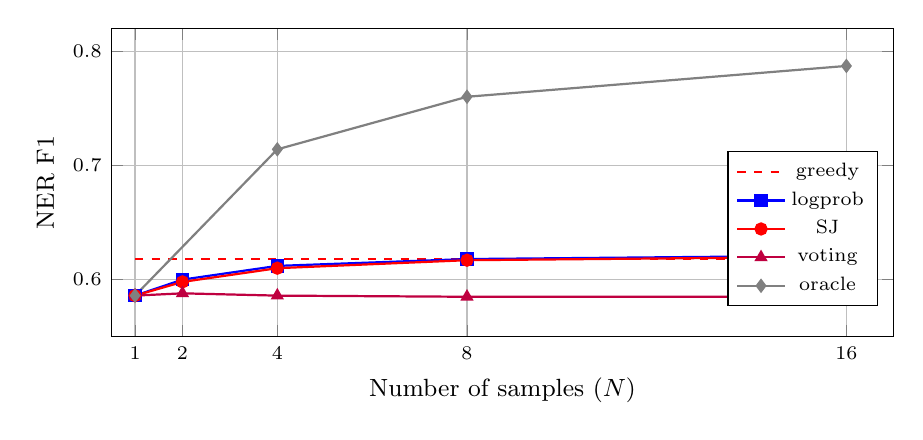
\begin{tikzpicture}
\begin{axis}[
  width=0.95\columnwidth, height=5.5cm,
  xlabel={Number of samples ($N$)},
  ylabel={NER F1},
  xmin=0.5, xmax=17, ymin=0.55, ymax=0.82,
  xtick={1,2,4,8,16},
  grid=major,
  legend style={at={(0.98,0.35)},anchor=east,font=\scriptsize},
  every axis label/.style={font=\small},
  tick label style={font=\scriptsize},
]
\addplot[thick, red, dashed, mark=none] coordinates {(1,0.618)(2,0.618)(4,0.618)(8,0.618)(16,0.618)};
\addlegendentry{greedy}

\addplot[thick, blue, mark=square*, mark size=2pt] coordinates {(1,0.586)(2,0.600)(4,0.612)(8,0.618)(16,0.621)};
\addlegendentry{logprob}

\addplot[thick, red, mark=*, mark size=2pt] coordinates {(1,0.586)(2,0.598)(4,0.610)(8,0.617)(16,0.620)};
\addlegendentry{SJ}

\addplot[thick, purple, mark=triangle*, mark size=2pt] coordinates {(1,0.586)(2,0.588)(4,0.586)(8,0.585)(16,0.585)};
\addlegendentry{voting}

\addplot[thick, black!50, mark=diamond*, mark size=2pt] coordinates {(1,0.586)(4,0.714)(8,0.760)(16,0.787)};
\addlegendentry{oracle}

\end{axis}
\end{tikzpicture}
\caption{Best-of-$N$ selection curves for SciERC NER. All unsupervised signals plateau near greedy performance (dashed red), while oracle grows monotonically, revealing a large unexploited headroom. Voting-based selection \emph{hurts} performance due to its instance-level nature.}
\label{fig:selection_curves}
\end{figure}

\subsection{$N$-Scaling and Seed Robustness}
\label{sec:nscaling}

Table~\ref{tab:nscaling} shows that increasing from $N{=}8$ to $N{=}16$ provides marginal improvement for NER SJ ($\rho$: $0.383 \to 0.398$) and is stable across three random seeds (mean $\rho{=}0.412 \pm 0.025$).
For RE, $N{=}16$ improves SJ from $\rho{=}0.211$ to $0.277$, but still falls short of the $0.40$ threshold achieved on NER.
The multi-seed stability (SD${=}0.025$) confirms our results are not artifacts of a particular random seed.

\begin{table}[t]
\centering
\small
\caption{$N$-scaling and seed robustness (SciERC, Qwen3-8B).}
\label{tab:nscaling}
\begin{tabular}{l cc cc}
\toprule
Config & NER SJ $\rho$ & RE SJ $\rho$ & NER AUROC & RE AUROC \\
\midrule
$N{=}8$, s42       & 0.383 & 0.244 & 0.689 & 0.592 \\
$N{=}16$, s42      & 0.398 & 0.277 & 0.697 & --- \\
$N{=}16$, s123     & 0.423 & 0.267 & --- & --- \\
$N{=}16$, s456     & 0.414 & 0.268 & --- & --- \\
\midrule
$N{=}16$ mean$\pm$SD & 0.412$\pm$0.025 & 0.271$\pm$0.006 & --- & --- \\
\bottomrule
\end{tabular}
\end{table}

\subsection{Ensemble Analysis}
\label{sec:ensemble}

Table~\ref{tab:ensemble} examines whether combining signals improves performance.
A logistic regression ensemble achieves NER AUROC of 0.735 (+0.7pp over best single signal voting\_conf), but fails to improve RE AUROC (0.719 vs voting alone 0.716).
The best linear combination is SJ+voting ($\alpha{=}0.3$) for NER ($\rho{=}0.489$) and voting+logprob ($\alpha{=}0.6$) for RE ($\rho{=}0.429$).
The SJ-logprob Pearson correlation is 0.57 (NER) and 0.42 (RE), indicating moderate complementarity.
Critically, even the ensemble \emph{cannot improve NER best-of-$N$ selection} (F1=0.604 vs greedy 0.609), reinforcing that the correlation-selection gap is fundamental, not a matter of signal strength.

\begin{table}[t]
\centering
\small
\caption{Ensemble analysis (SciERC, $N{=}8$).}
\label{tab:ensemble}
\begin{tabular}{l cc cc}
\toprule
& NER $\rho$ & NER AUROC & RE $\rho$ & RE AUROC \\
\midrule
Best single (voting) & 0.502 & 0.728 & 0.422 & 0.716 \\
Best linear combo    & 0.489 & --- & 0.429 & --- \\
Logistic ensemble    & --- & 0.735 & --- & 0.719 \\
\bottomrule
\end{tabular}
\end{table}

\subsection{Diagnostic Analysis: Why RE Is Harder}
\label{sec:diagnostic}

Table~\ref{tab:perrelation} reveals dramatic heterogeneity across relation types.
SJ achieves $\rho{=}0.545$ on HYPONYM-OF but $\rho{=}0.004$ on FEATURE-OF.
Fisher's Z-test confirms NER SJ $\rho$ is significantly higher than RE SJ $\rho$ ($p{=}0.021$), though bootstrap 95\% CIs overlap (NER: [0.295, 0.459]; RE: [0.142, 0.339]).

Entity span errors account for 55.5\% of RE false negatives, confirming compound error propagation: RE quality depends on correct entity extraction, and entity errors cascade into relation failures.
This explains why all confidence signals degrade on the full RE set but recover on the conditional set (where baseline entity extraction succeeds).

\begin{table}[t]
\centering
\small
\caption{Per-relation-type quality estimation (SciERC RE, Qwen3-8B). Large heterogeneity: $\rho_{\text{SJ}}$ ranges from 0.545 to 0.004.}
\label{tab:perrelation}
\begin{tabular}{l c ccc c}
\toprule
Relation & $n$ & $\rho_{\text{SJ}}$ & $\rho_{\text{FK}}$ & $\rho_{\text{VC}}$ & Mean F1 \\
\midrule
HYPONYM-OF   & 36  & \textbf{0.545} & 0.646 & 0.628 & 0.513 \\
CONJUNCTION  & 86  & 0.383 & 0.350 & 0.484 & 0.480 \\
USED-FOR     & 299 & 0.236 & 0.255 & 0.286 & 0.422 \\
PART-OF      & 44  & 0.239 & 0.348 & 0.283 & 0.297 \\
EVALUATE-FOR & 62  & 0.172 & 0.255 & 0.226 & 0.365 \\
COMPARE      & 35  & 0.168 & 0.184 & 0.180 & 0.453 \\
FEATURE-OF   & 50  & 0.004 & 0.052 & 0.014 & 0.254 \\
\bottomrule
\end{tabular}
\end{table}

\subsection{Temperature Sensitivity}
\label{sec:temperature}

SJ is highly robust to temperature: $\Delta\rho{=}\pm 0.01$ between $T{=}0.7$ and $T{=}1.0$, while FK shifts by $\pm 0.06$.
$T{=}1.0$ preserves more oracle headroom (RE: 0.167 vs 0.131 at $T{=}0.7$) and diversity ($1{-}\text{SJ}$: 0.389 vs 0.313), though no current signal can exploit this headroom.
Conditional filtering provides far larger improvements ($\Delta\rho{=}+0.07$ to $+0.14$) than temperature tuning---practitioners should prioritize filtering over temperature optimization.

\subsection{Capability Stratification}
\label{sec:stratification}

Stratifying instances by difficulty reveals that SJ is strongest on simple instances (entity count=0: $\rho{=}0.689$) and degrades on complex ones (entity count 3--5: $\rho{=}0.353$).
On hard RE instances (greedy F1$<$0.25), SJ correlation drops to $\rho{=}{-}0.043$---effectively random.
This confirms that consistency signals operate within the model's capability range and cannot rescue systematic failures.
An independent proxy analysis ($r{=}{-}0.021$ between sentence length and F1) verifies that our difficulty strata are not circular with the evaluation metric.

\subsection{OOD Robustness}
\label{sec:ood}

In out-of-domain evaluation (Appendix Table~\ref{tab:ood}), all signals degrade substantially (SJ: $\rho$ drops from 0.357 to 0.15), but structural signals maintain positive correlation while log-probability inverts ($\rho{=}{-}0.20$).
This has practical implications for closed-source API scenarios where log-probabilities are unavailable: structural consistency, despite weaker absolute correlation, provides directionally correct confidence estimates and does not actively mislead.

%=============================================================
\section{Practical Guidance}
\label{sec:practical}
%=============================================================

Based on our findings, we propose the following decision framework for practitioners:

\paragraph{When to use structural consistency (voting/SJ).}
For \emph{selective prediction} and \emph{abstention}: if the goal is to identify which instances are reliable (e.g., to route uncertain cases to human review), structural consistency provides the strongest signal (AUROC up to 0.73).
Also preferred when: (a)~log-probabilities are unavailable (closed-source APIs), (b)~domain shift is expected (structural signals degrade gracefully while logprob can invert), or (c)~temperature robustness is needed.

\paragraph{When to use log-probability.}
For \emph{best-of-$N$ selection} on tasks where greedy decoding is suboptimal (e.g., RE).
Log-probability is the only per-sample signal and the only one enabling effective sample selection in our experiments.

\paragraph{When neither helps.}
For NER best-of-$N$ selection with current models, greedy decoding is near-optimal---multi-sample generation provides no selection benefit despite large oracle headroom.
For tasks where the model systematically fails (e.g., social media NER with 54\% zero-F1 rate), no confidence signal is informative.

\paragraph{Voting vs.\ SJ.}
Entity voting is simpler, faster, and empirically stronger on full sets.
SJ generalizes to arbitrary structured outputs (relations, events) and is more temperature-robust.
For standard NER, voting is the practical default; for novel structured tasks or when temperature stability matters, prefer SJ.

%=============================================================
\section{Discussion}
\label{sec:discussion}
%=============================================================

\paragraph{The Correlation-Selection Gap as a General Phenomenon.}
Our finding that strong quality estimation does not imply effective selection may extend beyond IE.
Instance-level consistency signals inherently measure \emph{input difficulty}, not \emph{output quality variation} within a fixed input.
For tasks where within-input quality variance is low relative to between-input variance, the gap will be large.
Developing per-sample structural signals---not just instance-level aggregates---is a key direction for closing this gap.

\paragraph{Applicability to Closed-Source APIs.}
Many production IE systems use closed-source APIs (GPT-4, Claude) that do not expose log-probabilities.
In this setting, structural consistency signals offer unique value: they require only the generated text, not model internals.
Our OOD results (Section~\ref{sec:ood}) further suggest that log-probabilities can become \emph{anti-correlated} with quality under domain shift, making structural signals the safer default.

\paragraph{Limitations.}
(1)~We evaluate only 8B-parameter models; larger models may exhibit different patterns.
(2)~Both models are instruction-tuned; base models or fine-tuned models may differ.
(3)~We test on well-structured text domains (scientific, news); informal text (social media) remains unexplored---WNUT-17 was abandoned due to model capability failure.
(4)~RE evaluation is limited to SciERC; additional relational datasets would strengthen generalization claims.
(5)~We do not compare against supervised verifiers or reward models, which represent an upper bound on selection quality.

%=============================================================
\section{Conclusion}
\label{sec:conclusion}
%=============================================================

We present the first systematic comparison of unsupervised confidence signals for LLM-based information extraction, evaluating five signals across two tasks, two datasets, and two models.
Structural consistency signals (entity voting, soft Jaccard) provide the strongest instance-level quality estimation, substantially outperforming log-probability.
However, we identify a fundamental correlation-selection gap: no unsupervised signal beats greedy decoding for NER best-of-$N$ selection despite +16pp oracle headroom.
On relational tasks, compound error propagation degrades all signals, with dramatic per-relation heterogeneity.
We provide practical guidance distinguishing when to use structural consistency (selective prediction, closed-source APIs) vs.\ log-probability (sample selection on hard tasks), and characterize the task-complexity boundaries within which confidence estimation is reliable.

%=============================================================
\appendix
\section{OOD Robustness Details}
\label{app:ood}

\begin{table}[h]
\centering
\small
\caption{Out-of-domain robustness. Structural signals degrade but remain positive; log-probability inverts.}
\label{tab:ood}
\begin{tabular}{l cc c}
\toprule
Signal & In-Domain $\rho$ & OOD $\rho$ & $\Delta$ \\
\midrule
SJ      & 0.357 & 0.15  & $-$0.207 \\
FK      & 0.265 & 0.10  & $-$0.165 \\
logprob & 0.140 & $-$0.20 & $-$0.340 \\
\bottomrule
\end{tabular}
\end{table}

%=============================================================
\begin{thebibliography}{50}

\bibitem[Angelopoulos et~al.(2021)]{angelopoulos2021gentle}
A.~Angelopoulos et~al.
\newblock A gentle introduction to conformal prediction and distribution-free uncertainty quantification.
\newblock \emph{arXiv:2107.07511}, 2021.

\bibitem[Bates et~al.(2021)]{bates2021distribution}
S.~Bates et~al.
\newblock Distribution-free, risk-controlling prediction sets.
\newblock \emph{JASA}, 2021.

\bibitem[Brown et~al.(2024)]{brown2024large}
B.~Brown et~al.
\newblock Large language monkeys: Scaling inference compute with repeated sampling.
\newblock \emph{arXiv:2407.21787}, 2024.

\bibitem[Chen et~al.(2024)]{chen2024atomic}
Z.~Chen et~al.
\newblock Atomic self-consistency for better long form generations.
\newblock In \emph{EMNLP}, 2024.

\bibitem[Cobbe et~al.(2021)]{cobbe2021verifier}
K.~Cobbe et~al.
\newblock Training verifiers to solve math word problems.
\newblock \emph{arXiv:2110.14168}, 2021.

\bibitem[Culotta and McCallum(2004)]{culotta2004confidence}
A.~Culotta and A.~McCallum.
\newblock Confidence estimation for information extraction.
\newblock In \emph{HLT-NAACL}, 2004.

\bibitem[Derczynski et~al.(2017)]{derczynski2017wnut}
L.~Derczynski et~al.
\newblock Results of the WNUT2017 shared task on novel and emerging entity recognition.
\newblock In \emph{W-NUT}, 2017.

\bibitem[Desai and Durrett(2020)]{desai2020calibration}
S.~Desai and G.~Durrett.
\newblock Calibration of pre-trained transformers.
\newblock In \emph{EMNLP}, 2020.

\bibitem[Fisch et~al.(2021)]{fisch2021efficient}
A.~Fisch et~al.
\newblock Efficient conformal prediction via cascaded inference with expanded admission.
\newblock In \emph{ICLR}, 2021.

\bibitem[Gal and Ghahramani(2016)]{gal2016dropout}
Y.~Gal and Z.~Ghahramani.
\newblock Dropout as a {B}ayesian approximation: Representing model uncertainty in deep learning.
\newblock In \emph{ICML}, 2016.

\bibitem[Geifman and El-Yaniv(2017)]{geifman2017selective}
Y.~Geifman and R.~El-Yaniv.
\newblock Selective classification for deep neural networks.
\newblock In \emph{NeurIPS}, 2017.

\bibitem[Geng et~al.(2025)]{geng2025uqsurvey}
J.~Geng et~al.
\newblock A survey on uncertainty quantification for large language models.
\newblock In \emph{ACL Findings}, 2025.

\bibitem[Guo et~al.(2017)]{guo2017calibration}
C.~Guo et~al.
\newblock On calibration of modern neural networks.
\newblock In \emph{ICML}, 2017.

\bibitem[Hou et~al.(2025)]{hou2025uqcalibsurvey}
B.~Hou et~al.
\newblock A survey on uncertainty quantification and calibration for large language models.
\newblock \emph{arXiv:2503.15850}, 2025.

\bibitem[Huang et~al.(2025)]{huang2025cisc}
W.~Huang et~al.
\newblock {CISC}: Confidence-weighted self-consistency for improved reasoning.
\newblock In \emph{ACL Findings}, 2025.

\bibitem[Jagannatha and Yu(2022)]{jagannatha2022calibration}
A.~Jagannatha and H.~Yu.
\newblock Calibrating structured output predictors for natural language processing.
\newblock In \emph{ACL}, 2022.

\bibitem[Kadavath et~al.(2022)]{kadavath2022language}
S.~Kadavath et~al.
\newblock Language models (mostly) know what they know.
\newblock \emph{arXiv:2207.05221}, 2022.

\bibitem[Kossen et~al.(2024)]{kossen2024semanticprobes}
J.~Kossen et~al.
\newblock Semantic entropy probes: Robust and cheap hallucination detection in {LLM}s by exploiting {LLM} uncertainty.
\newblock \emph{arXiv:2406.15927}, 2024.

\bibitem[Kuhn et~al.(2023)]{kuhn2023semantic}
L.~Kuhn, Y.~Gal, and S.~Farquhar.
\newblock Semantic uncertainty: Linguistic invariances for uncertainty estimation in natural language generation.
\newblock In \emph{ICLR}, 2023.

\bibitem[Kuleshov and Liang(2015)]{kuleshov2015calibration}
V.~Kuleshov and P.~Liang.
\newblock Calibrated structured prediction.
\newblock In \emph{NeurIPS}, 2015.

\bibitem[Lakshminarayanan et~al.(2017)]{lakshminarayanan2017simple}
B.~Lakshminarayanan, A.~Pritzel, and C.~Blundell.
\newblock Simple and scalable predictive uncertainty estimation using deep ensembles.
\newblock In \emph{NeurIPS}, 2017.

\bibitem[Li et~al.(2026)]{li2026reasc}
Z.~Li et~al.
\newblock {ReASC}: Reliability-aware adaptive self-consistency.
\newblock \emph{arXiv:2601.02970}, 2026.

\bibitem[Lightman et~al.(2023)]{lightman2023stepwise}
H.~Lightman et~al.
\newblock Let's verify step by step.
\newblock \emph{arXiv:2305.20050}, 2023.

\bibitem[Liu et~al.(2025)]{liu2025rankedvoting}
Y.~Liu et~al.
\newblock Ranked voting self-consistency.
\newblock \emph{arXiv:2505.10772}, 2025.

\bibitem[Luan et~al.(2018)]{luan2018scierc}
Y.~Luan et~al.
\newblock Multi-task identification of entities, relations, and coreference for scientific knowledge graph construction.
\newblock In \emph{EMNLP}, 2018.

\bibitem[Manakul et~al.(2023)]{manakul2023selfcheckgpt}
P.~Manakul, A.~Liusie, and M.~Gales.
\newblock {SelfCheckGPT}: Zero-resource black-box hallucination detection for generative large language models.
\newblock In \emph{EMNLP}, 2023.

\bibitem[N{\'e}dellec and Xia(2026)]{nédellec2026consistency}
C.~N{\'e}dellec and F.~Xia.
\newblock Consistency--accuracy correlation in hard-prompted {LLM}s for entity and relation extraction.
\newblock \emph{Genomics Informatics}, 2026.

\bibitem[Shelmanov et~al.(2021)]{shelmanov2021uncertainty}
A.~Shelmanov et~al.
\newblock How certain is your {T}ransformer?
\newblock In \emph{EACL}, 2021.

\bibitem[Snell et~al.(2024)]{snell2024scaling}
C.~Snell et~al.
\newblock Scaling {LLM} test-time compute optimally can be more effective than scaling model parameters.
\newblock \emph{arXiv:2408.03314}, 2024.

\bibitem[Tjong Kim~Sang and De~Meulder(2003)]{tjong2003conll}
E.~Tjong~Kim~Sang and F.~De~Meulder.
\newblock Introduction to the {CoNLL}-2003 shared task: Language-independent named entity recognition.
\newblock In \emph{CoNLL}, 2003.

\bibitem[Vashurin et~al.(2025a)]{vashurin2025cocoa}
R.~Vashurin et~al.
\newblock {CoCoA}: Combining confidence and consistency for uncertainty quantification.
\newblock In \emph{NeurIPS}, 2025.

\bibitem[Vashurin et~al.(2025b)]{vashurin2025systematic}
R.~Vashurin et~al.
\newblock A systematic evaluation of {LLM} uncertainty quantification methods.
\newblock \emph{arXiv:2510.20460}, 2025.

\bibitem[Wang et~al.(2023)]{wang2023selfconsistency}
X.~Wang et~al.
\newblock Self-consistency improves chain of thought reasoning in language models.
\newblock In \emph{ICLR}, 2023.

\bibitem[Wu et~al.(2025)]{wu2025latentsc}
H.~Wu et~al.
\newblock Latent self-consistency.
\newblock \emph{arXiv:2508.18395}, 2025.

\bibitem[Xiao and Wang(2019)]{xiao2019uncertainty}
Y.~Xiao and W.~Wang.
\newblock Quantifying uncertainties in natural language processing tasks.
\newblock In \emph{AAAI}, 2019.

\bibitem[Xiong et~al.(2024)]{xiong2024confestimation}
M.~Xiong et~al.
\newblock Can {LLM}s express their uncertainty? An empirical evaluation of confidence elicitation in {LLM}s.
\newblock In \emph{NAACL}, 2024.

\bibitem[Yoshikawa et~al.(2025)]{yoshikawa2025abstention}
H.~Yoshikawa et~al.
\newblock Know your limits: A survey of abstention in large language models.
\newblock \emph{TACL}, 2025.

\bibitem[Zhang et~al.(2026)]{zhang2026selfcertainty}
S.~Zhang et~al.
\newblock Self-certainty best-of-$N$.
\newblock In \emph{ICLR}, 2026.

\end{thebibliography}

\end{document}
